% Options for packages loaded elsewhere
\PassOptionsToPackage{unicode}{hyperref}
\PassOptionsToPackage{hyphens}{url}
\PassOptionsToPackage{dvipsnames,svgnames*,x11names*}{xcolor}
%
\documentclass[
]{article}
\usepackage{lmodern}
\usepackage{amsmath}
\usepackage{ifxetex,ifluatex}
\ifnum 0\ifxetex 1\fi\ifluatex 1\fi=0 % if pdftex
  \usepackage[T1]{fontenc}
  \usepackage[utf8]{inputenc}
  \usepackage{textcomp} % provide euro and other symbols
  \usepackage{amssymb}
\else % if luatex or xetex
  \usepackage{unicode-math}
  \defaultfontfeatures{Scale=MatchLowercase}
  \defaultfontfeatures[\rmfamily]{Ligatures=TeX,Scale=1}
\fi
% Use upquote if available, for straight quotes in verbatim environments
\IfFileExists{upquote.sty}{\usepackage{upquote}}{}
\IfFileExists{microtype.sty}{% use microtype if available
  \usepackage[]{microtype}
  \UseMicrotypeSet[protrusion]{basicmath} % disable protrusion for tt fonts
}{}
\makeatletter
\@ifundefined{KOMAClassName}{% if non-KOMA class
  \IfFileExists{parskip.sty}{%
    \usepackage{parskip}
  }{% else
    \setlength{\parindent}{0pt}
    \setlength{\parskip}{6pt plus 2pt minus 1pt}}
}{% if KOMA class
  \KOMAoptions{parskip=half}}
\makeatother
\usepackage{xcolor}
\IfFileExists{xurl.sty}{\usepackage{xurl}}{} % add URL line breaks if available
\IfFileExists{bookmark.sty}{\usepackage{bookmark}}{\usepackage{hyperref}}
\hypersetup{
  pdftitle={Student Guide to Success},
  pdfauthor={Lab PI: C. Stallings},
  colorlinks=true,
  linkcolor=Maroon,
  filecolor=Maroon,
  citecolor=Blue,
  urlcolor=blue,
  pdfcreator={LaTeX via pandoc}}
\urlstyle{same} % disable monospaced font for URLs
\usepackage[margin=1in]{geometry}
\usepackage{longtable,booktabs}
% Correct order of tables after \paragraph or \subparagraph
\usepackage{etoolbox}
\makeatletter
\patchcmd\longtable{\par}{\if@noskipsec\mbox{}\fi\par}{}{}
\makeatother
% Allow footnotes in longtable head/foot
\IfFileExists{footnotehyper.sty}{\usepackage{footnotehyper}}{\usepackage{footnote}}
\makesavenoteenv{longtable}
\usepackage{graphicx}
\makeatletter
\def\maxwidth{\ifdim\Gin@nat@width>\linewidth\linewidth\else\Gin@nat@width\fi}
\def\maxheight{\ifdim\Gin@nat@height>\textheight\textheight\else\Gin@nat@height\fi}
\makeatother
% Scale images if necessary, so that they will not overflow the page
% margins by default, and it is still possible to overwrite the defaults
% using explicit options in \includegraphics[width, height, ...]{}
\setkeys{Gin}{width=\maxwidth,height=\maxheight,keepaspectratio}
% Set default figure placement to htbp
\makeatletter
\def\fps@figure{htbp}
\makeatother
\setlength{\emergencystretch}{3em} % prevent overfull lines
\providecommand{\tightlist}{%
  \setlength{\itemsep}{0pt}\setlength{\parskip}{0pt}}
\setcounter{secnumdepth}{5}
\usepackage{booktabs}
\ifluatex
  \usepackage{selnolig}  % disable illegal ligatures
\fi
\usepackage[]{natbib}
\bibliographystyle{apalike}

\title{Student Guide to Success}
\author{Lab PI: C. Stallings}
\date{Updated: 2020-11-03}

\begin{document}
\maketitle

{
\hypersetup{linkcolor=}
\setcounter{tocdepth}{2}
\tableofcontents
}
\hypertarget{the-fish-ecology-lab}{%
\section*{\texorpdfstring{\textbf{The Fish Ecology Lab}}{The Fish Ecology Lab}}\label{the-fish-ecology-lab}}

Welcome to the Fish Ecology Lab at the USF College of Marine Science! Making the transition from being an undergrad to a graduate student can be both rewarding and exciting, but also has its challenges. Although you are considered a graduate ``student,'' you will be treated like a professional. Thus, you will have to balance being a student and developing your skills (after all, that's why you are here), while also being treated as a colleague in the profession. This means that you will learn many new techniques and skills, but are expected to take charge of your learning and be the master of your own path. You will begin to contribute novel information to your scientific field. This guide is intended to help you make this transition so that you can excel here at USF and prepare yourself for a successful and rewarding career. I request that you review this handbook at the beginning of every semester since some advice is specific to different stages of your time as a graduate student.

You should also read and understand the CMS Student Handbook: \href{https://usf.app.box.com/s/2ew6pwdre3jkexgv8fgdwo8ticnvr7cc}{Master's Student} or \href{https://usf.app.box.com/s/mapv44nebi90iz7y9rjprsekcwps1yua}{Doctoral Student}

Additional information is also available from the \href{https://www.usf.edu/graduate-studies/}{USF Office of Graduate Studies}.

\begin{center}\rule{0.5\linewidth}{0.5pt}\end{center}

Contributors:\\
\emph{Timothy Pusack, Kara Wall, Dinorah Chacin, Ileana Freytis-Ortiz, etc.}

\begin{center}\rule{0.5\linewidth}{0.5pt}\end{center}

\hypertarget{suggested-timeline}{%
\section{\texorpdfstring{\textbf{Suggested Timeline}}{Suggested Timeline}}\label{suggested-timeline}}

\textbf{Integrated Marine Science Exam} (IMSE; \emph{optional})

\begin{itemize}
\tightlist
\item
  Recommended at the end of the second semester
\item
  Optional comprehensive exam across the four core disciplines of oceanography
\end{itemize}

\textbf{Committee formation}

\begin{itemize}
\tightlist
\item
  Recommended by the end of the second semester
\end{itemize}

\textbf{Prospectus} (i.e., proposal)

\begin{itemize}
\tightlist
\item
  By the end of the third semester; includes written and oral components delivered to your committee (also see Scheduling of Written Products)
\end{itemize}

\textbf{Candidacy qualifying exams} (PhD students)

\begin{itemize}
\tightlist
\item
  By the end of the sixth semester
\end{itemize}

\textbf{Defense} (also see Scheduling of Written Products)

\begin{itemize}
\tightlist
\item
  Master's Student: typically by sixth semester
\item
  Doctoral Student: typically by tenth semester
\end{itemize}

\textbf{Thesis/dissertation submission to Graduate School}

\begin{itemize}
\tightlist
\item
  Typically the same semester as defense (always after defense)
\item
  Be sure to check the deadlines with the Graduate School for thesis/dissertation submission and application for graduation
\end{itemize}

\emph{Notes: 1) That ``semesters'' here apply to fall and spring only, not summers, although you are expected to work in the summer. 2) that although this isn't a strict timeline, it gives an idea of where you should be at different stages of your graduate career}

\hypertarget{general-expectations}{%
\section{\texorpdfstring{\textbf{General Expectations}}{General Expectations}}\label{general-expectations}}

\hypertarget{read-read-read}{%
\subsection{Read, read, read}\label{read-read-read}}

Scholarship in science revolves around communication of findings, and the most efficient way to do this is by reading the literature. Learn how to read scientific literature and enjoy the process. Over the course of grad school, you will read thousands of papers (at least you should). At times you will read 4-5 papers per day. Know the literature.Know the classics. Know the frontier of your topics. I will provide you a list of books and peer-reviewed articles you're required to read, but this is just to get you started. When you're reading a paper, make note of cited papers that grab your interest and then read those. Have fun exploring papers during literature searches (I suggest using Web of Science, but some also like Google Scholar). Keep up with new literature by subscribing to both Tables of Contents of your favorite journals and Topics of Choice \ldots read, read, read!

\hypertarget{write-write-write}{%
\subsection{Write, write, write}\label{write-write-write}}

Scientific writing is a skill that needs to be developed and refined. The only way to get better at it is to write a lot. A major component of writing is editing. Learning to edit your writing as well as that of others is very important. Write often and exchange your written products with other students to receive feedback. Before giving a written product to me, it should go through three external edits by other students (This is the ``Three Then Me'' rule). Learn to receive constructive (err negative) feedback and use it to improve your writing and develop your skills. I don't expect you to be a perfect scientific writer when you start, but I do expect you to learn from your mistakes and minimize the occurrence of those as you progress through graduate school.

\hypertarget{quantitative-skills}{%
\subsection{Quantitative skills}\label{quantitative-skills}}

The backbone of science is math and statistics. Take as many stats courses as you can. Your analytical tool box will grow as you take more classes and these may inspire you to create new studies. Biometry and Multivariate Stats are often the most relevant to our lab, but there are others offered at CMS such as Data Analysis Methods (Time Series Analysis) and Ecosystem Modeling. You will never have as good of an opportunity as now to sharpen your quantitative skills. It's a lot harder to gain those skills after you graduate.

\emph{Note: I suggest you learn the R programming language; R is open source and has largely become the industry standard, so learning it now will pay off later when you have a job}

\hypertarget{soft-skills}{%
\subsection{Soft skills}\label{soft-skills}}

Soft skills include communication, interpersonal relationships, management, and leadership skills. Take advantage of your position as a graduate student to develop these in your time here. For example, take the lead on a group project or publication, write an opinion piece for the local newspaper (but please run by me first if you are doing it as a representative of USF CMS), or participate in the lab's outreach efforts (managing social media, participating in the Science Festival, etc.).

\hypertarget{regular-goals}{%
\subsection{Regular goals}\label{regular-goals}}

Complete weekly goal and productivity forms. An important skill to develop is to be able to set and meet your own deadlines. Hold yourself accountable for your own progress. When you first begin grad school, I'll ask for these each week and we'll review together. As you progress, we can back off to bi-weekly or monthly updates.

\emph{Note: You will also review how well I am doing as your advisor so that we can continue to improve our working relationship and productivity}

\hypertarget{work-space}{%
\subsection{Work space}\label{work-space}}

Learn to work in your office (or somewhere on campus where I can find you), not at home. There are several reasons for this.

\begin{enumerate}
\def\labelenumi{\arabic{enumi})}
\tightlist
\item
  I often need to talk to my students, whether to ask questions, present an opportunity, or respond to an inquiry.
\item
  Other faculty may also need to access you for the same.
\item
  Working at home isolates you from collaboration (e.g., water cooler chats that turn into papers or proposals).
\item
  In most jobs, you will be required to work at work, not at home, so you should become effective at doing so now.
\item
  For most people, working at home is distracting, resulting in reduced productivity.
\end{enumerate}

\emph{Note: If you struggle to work on campus, please talk to me about it so we can find a solution.}

\hypertarget{be-communicative}{%
\subsection{Be communicative}\label{be-communicative}}

Responsiveness to emails and other communications is important. We live in an era of nearly instant communication. Whether for good or bad, the professional world expects fairly rapid responses to emails. However, do not succumb to the email monster and be a slave to email. If you wait more than 48 hours to respond to an email, it may be interpreted as though you are ignoring it. And that's not good. If you need time to digest an email before you respond, simply reply back that you have read it and will soon respond once you're able to give it some thought. It's also good practice to confirm receipt of notifications or attachments so the sender knows you got them. I suggest setting two to three time blocks a day to respond to emails. This way you have time to focus on emails during those blocks and other time to focus on other tasks.

Communication is key. To have a successful graduate career and beyond it is important that we have a good working relationship. This means having open communication about your research, any problems/concerns, and exciting findings that you have. You are here to learn. If you don't know something, ask. Remember, you are a student. I don't expect you to know everything. The better I get to know you, and you get to know me, the more successful you will be. Please keep lines of communication open and make sure I am aware of how things are going for you. I want you to succeed. I will be one of your biggest advocates.

\hypertarget{be-passionate}{%
\subsection{Be passionate}\label{be-passionate}}

Find your excitement and passion. Finishing either a masters or a doctorate requires a lot of energy, time, and commitment. Make sure you are excited about your Thesis/ Dissertation. Take time to reflect on which topics you are excited about and which skills you are excited to use. These may change as time goes on and it is important to be honest with yourself about you interests. This does not mean constantly changing your focus or techniques used, but rather to focus your topic and hone your skills that you enjoy doing.

\hypertarget{time-management}{%
\subsection{Time management}\label{time-management}}

Put in the time. It's hard to be successful in grad school if you treat it like a M-F, 9-5 job. 40 hours per week usually won't cut it. I can't tell you that you must work XX hours per week. You'll need to figure that out on your own. But I can tell you that in grad school I put in at least 60 hours per week and often up to 80.

Punctuality is also very important. I shouldn't have to point this out, but the culture in academia can sometimes be a bit gray on this. Even being one minute late sends the wrong message. When you are late, you send a message to those waiting on you that your time is more important than theirs. Conversely, arriving on time or even a few minutes early reflects that you are engaged and interested and value the purpose of the meeting. This applies to everything involving a set meeting time, whether it's a class, field work, lab meetings, meetings with a colleague, etc.

Deadlines are the reality of the career you have chosen (and most careers for that matter). Take them seriously. This of course applies to deadlines established externally (e.g., due date of a fellowship application), but also internally with colleagues (e.g., getting a ms draft to me).

Be judicious with your time commitments. During graduate school you will have the opportunity to join many groups, contribute to many collaborations, and partake in many projects. However, this can lead to over commitment. An important skill to develop is the ability to say ``no'' to certain opportunities and know which ones to say ``no'' to. The ultimate goal of graduate school is to graduate; therefore, make sure the majority of your time is dedicated towards those tasks required to graduate (required classes, examinations, research, and publishing).

\hypertarget{data-analyses}{%
\section{\texorpdfstring{\textbf{Data \& Analyses}}{Data \& Analyses}}\label{data-analyses}}

\hypertarget{organization}{%
\subsection{Organization}\label{organization}}

You will create, acquire, and accumulate an enormous amount of files during grad school and much, much more throughout your career. So it is truly imperative to establish a good file naming system and a good folder system for storing everything. The best systems will not only make sense to you, but could also be easily navigable to others. This document is an excellent and simple guide for naming files: \href{https://docs.google.com/presentation/d/1NqfzjMlilJzXKUujFkzSr7xc1eKlDj5TVy02Zg8opwg/present?slide=id.p}{Data Science of Marine Conservation}

\begin{figure}

{\centering 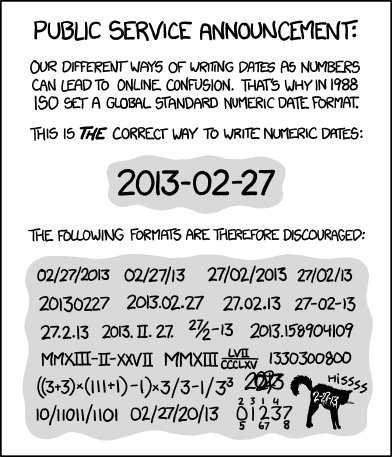
\includegraphics[width=0.75\linewidth]{Images/FileDating_YYYY_MM_DD} 

}

\caption{Seriously, include the date in your files and use the International Organization for Standardization (ISO) format.}\label{fig:unnamed-chunk-1}
\end{figure}

\hypertarget{shared-folders}{%
\subsection{Shared folders}\label{shared-folders}}

We will use a file/folder sharing system in the FEL. Currently, that system is Box. This will be used for group projects as well as one-on-one sharing with Stallings.

For the one-on-one parent folder, there will four subfolders:

\begin{itemize}
\tightlist
\item
  \textbf{Funding}: this will have subfolders for every scholarships, fellowship, etc that you apply for. The subfolders will house the funding instructions, application, CV, etc.
\item
  \textbf{General}: this is a catch-all subfolder for items that don't quite fit in with the other subfolders.
\item
  \textbf{Presentations}: this will have subfolders for each presentation you give at meetings and seminars.
\item
  \textbf{Thesis}: this folder will house all your thesis-based data and products. There will be subfolders for each chapter, the proposal (including the proposal presentation here instead of the presentations folder), data, code for analysis, and the defense presentation (here instead of the presentations folder)
\end{itemize}

\hypertarget{analytical-tools}{%
\subsection{Analytical tools}\label{analytical-tools}}

I strongly encourage you to use R. Regardless of the programming language you choose, having good data management and workflow is critical.

\begin{itemize}
\tightlist
\item
  Please read this really nice guide:

  \begin{itemize}
  \tightlist
  \item
    \href{https://journals.plos.org/ploscompbiol/article?id=10.1371/journal.pcbi.1005510}{Good enough practices in scientific computing}
  \end{itemize}
\item
  Getting started in R:

  \begin{itemize}
  \tightlist
  \item
    \href{https://stat545.com/}{Stat545}
  \item
    \href{https://r4ds.had.co.nz/}{R for Data Science}
  \item
    \href{https://rstats.wtf/}{What they forgot to teach you about R}
  \end{itemize}
\item
  Version control:

  \begin{itemize}
  \tightlist
  \item
    \href{https://peerj.com/preprints/3159.pdf}{Excuse me, do you have a moment to talk about version control?}
  \item
    \href{https://happygitwithr.com/index.html}{Happy Git and GitHub for the useR}
  \end{itemize}
\end{itemize}

\hypertarget{production-and-communication}{%
\section{\texorpdfstring{\textbf{Production and Communication}}{Production and Communication}}\label{production-and-communication}}

Publish, publish, publish (publish or perish!). Publications are the currency in our field. Journal quality is very important, especially for PhD students hoping to get a job! Think Ecology, Ecology Letters, etc.

\begin{itemize}
\tightlist
\item
  MS students: a minimum of two publishable papers from thesis
\item
  PhD students: a minimum of three publishable papers from dissertation (should be highly interrelated studies that when synthesized should advance our understanding about an important topic)
\end{itemize}

\hypertarget{writing-a-manuscript}{%
\subsection{Writing a manuscript}\label{writing-a-manuscript}}

\emph{Note: Try starting with ``outline'' view in word processor}

\begin{enumerate}
\def\labelenumi{\arabic{enumi})}
\tightlist
\item
  Layout all \textbf{FIGURES} and \textbf{TABLES}

  \begin{itemize}
  \tightlist
  \item
    Determine what to include to tell a complete story.
  \end{itemize}
\item
  Write the \textbf{RESULTS} first

  \begin{itemize}
  \tightlist
  \item
    What you found (this is a fairly easy section to write).
  \end{itemize}
\item
  Next, write the \textbf{METHODS}

  \begin{itemize}
  \tightlist
  \item
    How did you produce the results you just described?
  \end{itemize}
\item
  Then write the \textbf{DISCUSSION}

  \begin{itemize}
  \tightlist
  \item
    What do those results mean?
  \end{itemize}
\item
  Finally, write the \textbf{INTRODUCTION}

  \begin{itemize}
  \tightlist
  \item
    Set the stage for the results and inference that came from the study.
  \end{itemize}
\item
  Wrap up by writing \textbf{ABSTRACT} with about two key sentences from each section.
\end{enumerate}

Regarding \textbf{KEYWORDS}: don't use keywords that show up in your title or abstract. The search engines will find them, so putting them in keywords list is redundant, a waste of limited keywords, and limits the number of hits your paper will get.

This is an excellent resource for structuring your manuscript: \href{https://www.elsevier.com/connect/11-steps-to-structuring-a-science-paper-editors-will-take-seriously}{11 Steps to Structuring a Science Paper}

\hypertarget{writing-skills}{%
\subsection{Writing skills}\label{writing-skills}}

Learn how to become a self-editor (see our lab's writing cheat sheet and always keep Strunk and White nearby). You should be your toughest critic, not me. Ask whether you have given complete and balanced treatment of the topic. Is the writing well-organized and written in scholarly language? Are the mechanics correct?

I edit heavily. Learn from manuscript edits, don't just accept track changes. Compare what you wrote to the edits I made. Understand why the changes were made. If you don't, ask me (or whoever made edits). It's ok to disagree. It's not ok to ignore. The intention is to:

\begin{enumerate}
\def\labelenumi{\arabic{enumi})}
\tightlist
\item
  Improve the quality of the product
\item
  More importantly, teach you how to become an effective writer.
\end{enumerate}

We follow the CMS's \href{https://www.usf.edu/marine-science/about-us/college-documents.aspx/}{Code of Conduct} regarding the expected time it takes to publish work derived from your time here, regardless of whether you are an undergraduate intern, graduate student (MS or PhD), postdoc, or visiting scientist. Specifically, the Code of Conduct states: ``Sometimes a student's work must be published very quickly and before they graduate (e.g., due to grant restrictions or because it is a novel work that might be ``scooped'' if not published quickly). However, if the advisor agrees that it is not necessary to publish the work immediately, then a graduated student can publish the work as first author within a reasonable time after completing their degree. The exact amount of time must be agreed upon by both the student and the advisor. If a graduated student does not make a good-faith attempt to submit their research for publication within the time frame mutually agreed upon by the student and advisor, AND the advisor has either documented written attempts to contact the student about the manuscript or confirmed that the work has been abandoned by the student, then the advisor assumes the right to publish parts or all of that thesis or dissertation research as first author (or ask another student, post-doc, or staff member to take over the manuscript). In this case, the graduated student will be listed as a co-author as appropriate to their contributions to a publication.''

Present research at symposia, conferences, etc. Our lab frequently attends the Benthic Ecology Meeting (usually mid-late March), and sometimes ESA, AFS (national), AFS (Florida), GCFI, ICES, WSN, ASLO, and others.

\begin{itemize}
\tightlist
\item
  All presentations (oral and posters) must first be presented to lab for a practice run and feedback.
\item
  Practice run must occur at least one week before conference presentation.
\item
  Presentation should be polished at time of practice run. Don't apologize and say you haven't practiced it yet -- what's the point of us editing it at that stage?
\item
  For the practice run, presenter is responsible for reserving the space (usually in lab), projector, and scheduling attendance.
\end{itemize}

\hypertarget{authorship}{%
\subsection{Authorship}\label{authorship}}

In peer-review publications and presentations included as part of a thesis or dissertation, I should be listed as the last author as I am the PI of the laboratory where the investigation has been conducted. If publications or presentations are the product of a research collaboration with another laboratory or research group where funding or any other source of assistance is provided, a meeting prior to the initiation of the project should be held in order to decide authorship order and responsibilities. Additional individuals who contributed substantially to the design, acquisition, analysis, or interpretation of the data, and drafting of manuscript should be listed as co-authors. I also encourage you to participate in side-projects, whether they involve me or not. For any non-thesis related publications of which I have not participated, I do not expect authorship.

\hypertarget{scheduling-of-written-products}{%
\section{\texorpdfstring{\textbf{Scheduling of Written Products}}{Scheduling of Written Products}}\label{scheduling-of-written-products}}

\hypertarget{prospectus-thesis-and-dissertation}{%
\subsection{Prospectus, thesis, and dissertation}\label{prospectus-thesis-and-dissertation}}

\begin{itemize}
\tightlist
\item
  Check with the Graduate School or Sami to get the ETD deadline for the semester you are planning to graduate. Plan your defense a minimum of THREE weeks prior to the ETD deadline to allow time for edits before it is due.
\item
  Give me a very polished version of the ms EIGHT WEEKS before committee meeting (see above about Three Then Me). This allows time for one to two edits between you and me before submitting to committee.
\item
  Give the edited ms to your entire committee FOUR WEEKS before committee meeting. This allows your committee to have two weeks prior to the mandatory Sufficiency Meeting, which has to occur at least two weeks prior to your defense.
\end{itemize}

\hypertarget{how-to-schedule-a-committee-meeting}{%
\subsection{How to schedule a committee meeting}\label{how-to-schedule-a-committee-meeting}}

\begin{itemize}
\tightlist
\item
  First, understand that your committee members are all very busy, so scheduling a meeting far in advance (i.e., 2-3 months) is key
\item
  Once you have a target time window of 2-3 weeks, check with Chris for availability. Then, based on his availability, send an email to your committee to ask for their general availability during that time. Will they be around or traveling?
\item
  Check with Flo for room availability. We usually hold proposal, doctoral candidacy, defense meetings in the MSL Conference Room. It's best to hold it there for defenses, but we have other options from proposal meetings and candidacy exams (e.g., COT Conf Room, KRC Second Floor Conf Room).
\item
  Once you have narrowed down some dates that work for everyone and with available meeting space, create a Doodle poll (or any similar service) with time slots and dates for them to choose from.
\end{itemize}

\emph{Notes: 1) Stay on top of this process to move it along swiftly. Someone may at first be available on a particular day, but if you don't lock it in with a set meeting day and time for them to mark on their calendar, their availability may change. 2) You are in charge of reserving the meeting space. Please reserve the room for a total of 3.5 hours, thereby allowing for 30 minutes prior to the meeting and then 3 hours for it.}

\hypertarget{funding-proposals}{%
\subsection{Funding proposals}\label{funding-proposals}}

For both external and internal CMS fellowships:

\begin{itemize}
\tightlist
\item
  Begin early! This is especially important for the highly competitive sources such as NSF.
\item
  Get a polished draft of proposal to me at least \textbf{four weeks} before deadline (again, see above about Three Then Me).
\item
  Notify letter writer of request at least \textbf{two weeks} before deadline
\item
  When asking for the letter, provide the writer

  \begin{enumerate}
  \def\labelenumi{\alph{enumi})}
  \tightlist
  \item
    The description of fellowship, job, etc. (including documentation, web links, etc.)
  \item
    Your CV,
  \item
    Your application including any proposal or research statement materials
  \item
    Qualities you want the writer to highlight in the letter (the more ammo you can give the writer, the better they can do to write a very strong letter)
  \end{enumerate}
\end{itemize}

\emph{Note: It is typically expected that your major professor will be one of your letter writers during grad school and even years after it}

\hypertarget{scheduling-and-preparing-for-meetings}{%
\section{\texorpdfstring{\textbf{Scheduling and preparing for meetings}}{Scheduling and preparing for meetings}}\label{scheduling-and-preparing-for-meetings}}

\hypertarget{meeting-format}{%
\subsection{Meeting Format}\label{meeting-format}}

\textbf{Proposal}:

\begin{itemize}
\tightlist
\item
  Ideally this are a round-table style discussion with the intension of making sure your questions and study design are logical, based on solid scientific premise, possible to accomplish in a graduate school time frame, and will result in high-quality publications. You will prepare a 10-15 minute presentation on your proposal with a standard introduction to the topics and concepts, study questions, study design, predictions (if possible -- and they should be), and a timeline.
\end{itemize}

\textbf{PhD Comps} (Candidacy):

\begin{itemize}
\tightlist
\item
  Believe it or not, I found my candidacy exam to be one of the most fulfilling aspects of my graduate training. You will never have this amount of time to dedicate to reading and sharpening your expertise in your field of study. For the exam, we typically have two rounds of questions with the first round fairly specific to your research and the second round extending more broadly to see gauge the limits of your knowledge in the field. We all want you to do well. Try to have fun with it!
\end{itemize}

\textbf{Sufficiency}:

\begin{itemize}
\tightlist
\item
  The format from this meeting can be anything from everyone providing feedback over email to having a formal gathering. The goal here is to make sure there are no surprises at the defense from any committee members regarding their opinion of your research. I won't let you have this meeting until I think you are ready, so it should primarily be a formality.
\end{itemize}

\textbf{Defense}:

\begin{itemize}
\tightlist
\item
  You have made it to your defense! Congratulations, you have much to be proud of. You will prepare a 45-50 min presentation for the public (invite your friend, family, etc), followed by 10-15 min of Q\&A from them. We will then take a short 5-10 min break and then reconvene with the committee for the second part of the defense. Similar to the candidacy exam, each committee member can ask any question and there are usually 1-2 rounds of questions. Unlike the candidacy exam, the questions are usually fairly specific to your research, ways to improve the manuscripts for publication, and discussions about future research. Again, this is your day. Have fun with it!
\end{itemize}

\hypertarget{what-to-bring-to-a-committee-meeting}{%
\subsection{What to bring to a committee meeting:}\label{what-to-bring-to-a-committee-meeting}}

There are forms required for each meeting. Please check here for the most up to date links for them: \href{https://www.marine.usf.edu/education/current-students/forms/}{USF CMS Student Forms}. Please print the forms with appropriate information filled in for each (names for you and your committee members, date, etc.).

\textbf{Proposal meeting}:

\begin{itemize}
\tightlist
\item
  Committee Appointment Form (1 total),
\item
  Proposal SACS Eval Form (rubric; 1 for each committee member).
\end{itemize}

\emph{Note: You may (and probably should) have your committee sign the appointment form as soon as you form it as faculty receive teaching credit for the time served on your committee}

\textbf{PhD Comps} (Candidacy):

\begin{itemize}
\tightlist
\item
  Candidacy Approval Form (1 total)
\item
  PhD Comp Exam SACS Eval Form (rubric; 1 for each committee member).
\end{itemize}

\textbf{Sufficiency} (i.e., request for defense):

\begin{itemize}
\tightlist
\item
  Request for Defense Form (1 total)
\end{itemize}

\textbf{Defense}:

\begin{itemize}
\tightlist
\item
  Successful Defense Form (1 total)
\item
  Certificate of Approval (1 total),
\item
  Written SACS Eval Form (rubric; 1 for each committee member),
\item
  Defense SACS Eval Form (rubric; 1 for each committee member).
\end{itemize}

\emph{Note: For all meetings, I think it is a sign of appreciation for your committee's time to bring light refreshments}

\hypertarget{prospectus}{%
\section{\texorpdfstring{\textbf{Prospectus}}{Prospectus}}\label{prospectus}}

The prospectus should be as long as it needs to be to get your point across. There is no suggested length, as this depends on the project and the progress that has been made on the project. Most proposals fall in the range of 8-10 pages for MS and 10-15 for PhD.

\hypertarget{format}{%
\subsection{Format}\label{format}}

\textbf{Abstract} \emph{(optional)}

\begin{itemize}
\tightlist
\item
  There is a section on the SACS evaluation form for an abstract, but this is not necessary in a prospectus format.
\end{itemize}

\textbf{Introduction}

\begin{itemize}
\tightlist
\item
  This should include all information necessary to set up your specific questions that you plan to investigate in your thesis/dissertation with a fairly comprehensive literature review the demonstrates you have done your due diligence on the topic. The information presented should reflect a thorough understanding of your dissertation topic, and the research leading up to it. Your introduction should describe how your proposed study will fill a gap in the knowledge/research of your topic of interest or apply existing knowledge in a novel way (e.g., novel technique, new location).
\end{itemize}

\textbf{Research questions}

\begin{itemize}
\tightlist
\item
  The specific questions that are being asked through your project. These can be integrated into your introduction or exist as a separate section. If the questions are hypothesis-driven, state and detail the specific hypotheses that are being tested.
\end{itemize}

\textbf{Methodology}

\begin{itemize}
\tightlist
\item
  An overview of the methods that will be used for data collection and analysis. These should be broken down by the question of interest (or if general methodology, make a separate sub-section). Your methods should be detailed to the point where your committee understands what you're doing, but they do not need to be detailed to the extent of a manuscript. It is okay to not have all the answers at this point. Your committee will help you determine specific experimental/analytical methods if you are not certain as to the proper method to use.
\item
  If data will be obtained through a secondary source, provide details on the structure of the data and the methods used to collect them. This can be separated out into its own section or integrated into your methods.
\end{itemize}

\textbf{Progress to date}

\begin{itemize}
\tightlist
\item
  This section will vary depending on where each student is in their graduate career at the time of writing the prospectus, and on the nature of the project. Detail all steps that have been taken thus far in obtaining data, preliminary analyses, etc. If preliminary results are available, provide these through both prose and figures. Note, it is not necessary to have preliminary data and results at the time of writing the proposal.
\end{itemize}

\textbf{Academic timeline}\\
This should include the following milestones and the semester(s) of their projected completion:

\begin{itemize}
\tightlist
\item
  Committee formation
\item
  Proposal submission
\item
  Proposal meeting
\item
  Doctoral Candidacy Exam (PhD Only)
\item
  Major milestones for research project (data collection, analyses, etc.)
\item
  Thesis/dissertation writing (can also include manuscript submission)
\item
  Thesis/dissertation defense
\item
  Expected graduation
\end{itemize}

\textbf{Completed coursework}

\begin{itemize}
\tightlist
\item
  An updated schedule of all courses taken in grad school, their completion date, type (e.g., core, elective, MRA), and grade earned. This will allow your committee to identify potential gaps in your curriculum. Make note of courses that have not yet been completed but you plan to take, and their expected completion. If you are a PhD student, include the date of IMSE completion in this section.
\end{itemize}

\textbf{Literature cited}

\begin{itemize}
\tightlist
\item
  This should be a comprehensive list of all sources used in your prospectus. Internal citations should be of the form (Author Year).
\end{itemize}

\hypertarget{participation}{%
\section{\texorpdfstring{\textbf{Participation}}{Participation}}\label{participation}}

Attend lab meetings; almost NO exceptions unless you are sick, unavoidably in the field, or at a conference; if you have a job, schedule lab meetings at beginning of semester and work job around them (this includes FWRI and NOAA employees).

Assist labmates and me with field and lab work.

Participate in weekly updates on lab's social media (usually just 1-2 per semester).

Help keep lab webpage updated, including your personal webpage.

Attend CMS seminars, even when the topic is not related to your area of expertise. You might learn something cool\ldots at the very least, you have an opportunity to see many presentation styles and note what works well (and what doesn't).

\textbf{If you are sick, stay at home} \emph{Seriously.} Definitely stay away from me!

  \bibliography{book.bib,packages.bib}

\end{document}
